\chapter{Main Board}
\section{Introduction}
For project a common power supply and connection platform for all the robot parts has been designed. This board (figure \ref{fig:Main Board} ) should provide different levels of power supply for different purposes(motors, sensor, FPGA)and space  to connect all necessary hardware.
The input power supply has been set to 20 V,3 A.

\begin{figure}[!ht]
	\begin{subfigure}{.49\textwidth}
		\centering
		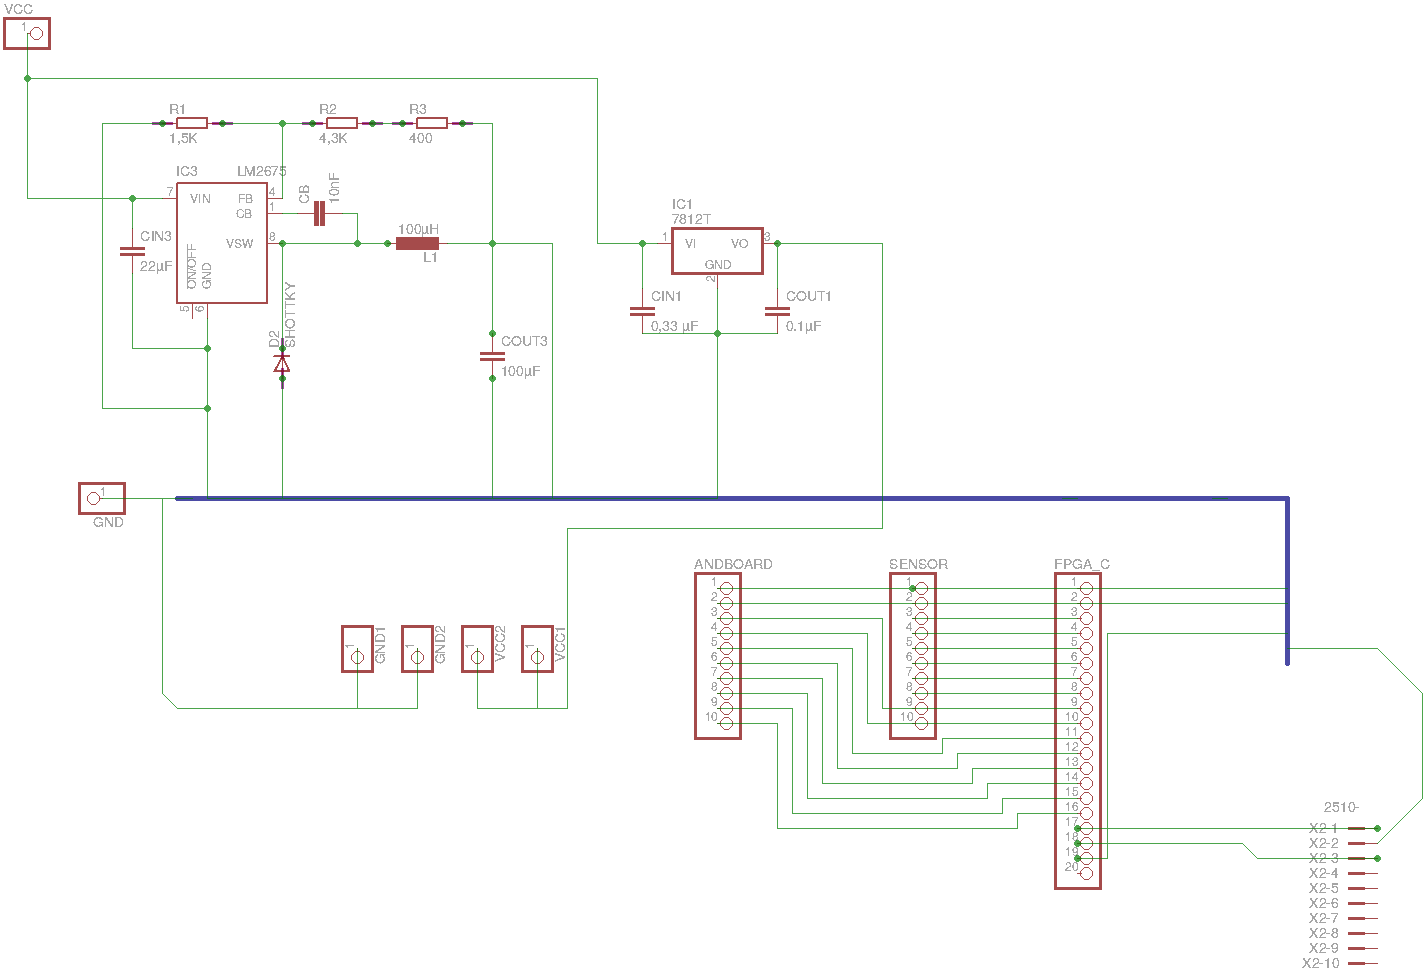
\includegraphics[width=1\textwidth]{figures/Main_board_schematics}
		\caption{Main Board schematics}
		\label{fig:MainSchematics}
	\end{subfigure}
	\begin{subfigure}{.49\textwidth}
		\centering
		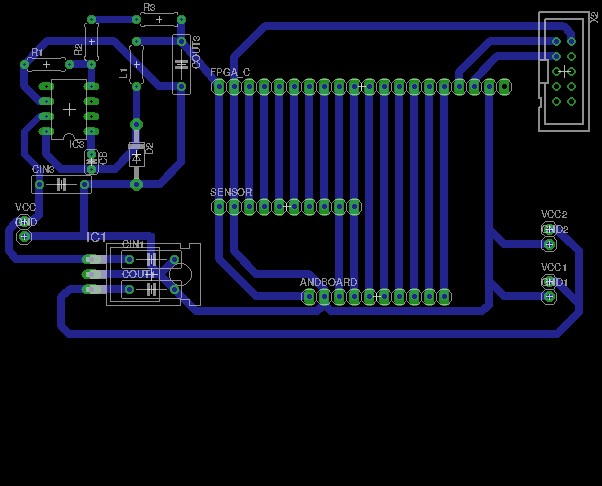
\includegraphics[width=1\textwidth]{figures/Main_board_brd}
		\caption{Main Board pcb}
		\label{fig:MainBRD}
	\end{subfigure}
\caption{Main Board}
\label{fig:Main Board}
\end{figure}

\section{Components choice and design implementation}

For the 12 V power supply,necessery for a correct operation of the motors, a linear voltage regulator LM7812 \cite{linear_regulator} has been employed,the circuit has been designed following the recommendation from the component data sheet. The linear regulators are low in effieciency, but easy to implement and with higher ripple rejection rates. The LM7812 is able to support up to 2 A of supply current which is sufficient for the motors employed.As shown in the recommended schematics,0.3 $\mu F$ input $C_{in}$ and 0.1  $\mu F$ output $C_{out}$ capacitors have been used. The chosen regulator embeds internal current limiting, thermal shut-down and safe area protection, making it essentially indestructible.

\begin{figure}[!ht]
	\centering
	\includegraphics[width=1.0\textwidth]{figures/linear_regulator}
	\caption{TS7812 regulator implementation}
	\label{fig:linear_reg}
\end{figure}
 
The maximum $V_{cc}$ for the chosen motors is 12 V.Through LM7812 linear regulator a stable 11.70 V,without any ripple (by the support from the used capacitors) has been obtained.This value could  have been raised to 12 V by adding an additional circuit, but the difference has been considered acceptable. 
 
Besides,a power supply for other components (ADC, distance sensor) and the FPGA has been designed.Through $LM2675N-ADJ Switching Regulator$ \cite{switching_regulator} has been possible implement a stable and energetically efficient 5 V power supply.Infact, switching regulators have a slightly difficult implementation, but are longer efficient than linear voltage regulators. According to the data sheet, its efficiency reaches up to 96 \%.Since the employed IC has an adjustable output,it offers the opportunity to obtain different range of output current ( 0.1 A-1 A) changing the value of the components in the following configuration.To implement the related circuit,the recommended guideline has followed to obtain 5 V,1 A output(for the sake of the shortness,instead of drawing out with description,it has been attached in the appendix).

\begin{figure}[!ht]
	\centering
	\includegraphics[width=1.0\textwidth]{figures/switching_regulator}
	\caption{Switching regulator implementation}
	\label{fig:linear_reg}
\end{figure}

The final board contains both power supply lines.Furthermore,it hosts pin connectors to connect the different add-ons (H-bridges drive, sensor board, FPGA, uTosNet. The board has been carefully designed in order to minimize the sizes and save space. 
\newpage 
\section{Conclusions}
The main board,is fully capable of power supplying the motors and also the FPGA, sensor and ADC (5 V).Furthermore it hosts an interface to connect different board and the uTosNet connection. 